\section{Ejemplo manual}\label{sec:manual}

\subsection{Datos}
Se usa una ruta pequeña con \textbf{3 buses} y \textbf{8 vueltas} de duración base \textbf{90\,min} (cercana a la de RTI-08, 1.57\,h, redondeada para calcular a mano). Los almuerzos inician en: B1 entre 10:30 y 11:30, B2 entre 12:00 y 13:00, y B3 entre 13:30 y 14:30. Se usa el perfil de tráfico \textbf{T2}, que tiene factores redondos.

\begin{table}[H]
\centering\small
\caption{Vueltas de la instancia manual y su tiempo de viaje (min) con tráfico T2.}\label{tab:manual-datos}
\begin{tabular}{cccccc}
\toprule
Vuelta & \makecell{Duración\\base $\pbar_j$} & \makecell{Ventana\\de inicio} & \makecell{$p_j$ si sale\\en $r_j$} & \makecell{$p_j$ si sale\\en $d_j$} & \makecell{$p_j$ en la\\salida nominal} \\
\midrule
J1 & 90 & 06:00--06:30 & 103.7 & 117.0 & 110.3 \\
J2 & 90 & 06:30--07:00 & 117.0 & 117.0 & 117.0 \\
J3 & 90 & 07:00--07:30 & 117.0 & 110.8 & 114.2 \\
J4 & 90 & 08:00--08:30 & 103.8 & 96.9 & 100.4 \\
J5 & 90 & 09:30--10:30 & 90.0 & 90.0 & 90.0 \\
J6 & 90 & 11:30--12:30 & 102.0 & 108.0 & 108.0 \\
J7 & 90 & 16:30--17:00 & 111.0 & 121.5 & 116.3 \\
J8 & 90 & 17:00--17:30 & 121.5 & 121.5 & 121.5 \\
\bottomrule
\end{tabular}
\end{table}

\subsection{Cálculo del tiempo de viaje con tráfico}
\textbf{J1 saliendo a las 06:00.} La franja 06:00--06:30 ($f = 0.9$) dura 30\,min reales y cubre $30/0.9 = 33.33$\,min base. Faltan 56.67\,min base, que en la punta mañana ($f = 1.3$) toman $56.67 \times 1.3 = 73.67$\,min. Entonces $p_{J1}(06{:}00) = 30 + 73.67 = \mathbf{103.67}$\,min y la llegada es a las 07:43.7.

\textbf{J4 saliendo a las 08:00.} Hasta las 09:00 hay 60\,min reales a $f = 1.3$, que cubren 46.15\,min base; los 43.85 restantes van a $f = 1.0$. Entonces $p_{J4}(08{:}00) = 60 + 43.85 = \mathbf{103.85}$\,min.

\textbf{J4 saliendo a las 08:27.} Hasta las 09:00 hay 33\,min reales, que cubren 25.38\,min base; los 64.62 restantes van a $f = 1.0$. Entonces $p_{J4}(08{:}27) = 33 + 64.62 = \mathbf{97.62}$\,min. Salir más tarde dentro de la ventana reduce el tiempo de viaje porque se pasa menos tiempo en la punta.

\textbf{J7 saliendo a las 16:30.} Hasta las 17:00 hay 30\,min a $f = 1.0$; los 60\,min base restantes van a $f = 1.35$ y toman 81\,min. Entonces $p_{J7}(16{:}30) = \mathbf{111.0}$\,min.

\begin{nota}
\textbf{\color{guinda}Verificación.} La hoja \emph{Calculadora vuelta} del Excel reproduce este cálculo con fórmulas (06:00, 90\,min, T2 $\to$ 103.67\,min) y coincide con el programa.
\end{nota}

\captura[5.5cm]{excel_calculadora_vuelta.png}{Hoja \emph{Calculadora vuelta} del Excel: cálculo de $p_{J1}(06{:}00)$ con el perfil T2.}{fig:cap-calculadora}

\subsection{Asignación con List Scheduling}
Orden de la lista: J1, J2, \dots, J8 (por inicio de ventana). En cada paso se muestran, para cada bus, la salida y llegada factibles y la carga previa (min).

\begin{table}[H]
\centering\small
\caption{Traza de List Scheduling (T2). (*) B1 debe iniciar su almuerzo entre 10:30 y 11:30, por eso J6 solo cabe después del almuerzo.}\label{tab:traza-ls}
\footnotesize\setlength{\tabcolsep}{4pt}
\begin{tabular}{clllll}
\toprule
Paso & Vuelta & B1 & B2 & B3 & Elegido \\
\midrule
1 & J1 & 06:00--07:44 · 0 & 06:00--07:44 · 0 & 06:00--07:44 · 0 & \textbf{B1} (empate $\to$ índice) \\
2 & J2 & infactible & 06:30--08:27 · 0 & 06:30--08:27 · 0 & \textbf{B2} \\
3 & J3 & infactible & infactible & 07:00--08:57 · 0 & \textbf{B3} \\
4 & J4 & 08:00--09:44 · 103.7 & 08:27--10:05 · 117.0 & infactible & \textbf{B1} (menor carga) \\
5 & J5 & 09:44--11:14 · 207.5 & 09:30--11:00 · 117.0 & 09:30--11:00 · 117.0 & \textbf{B2} (empate $\to$ índice) \\
6 & J6 & 12:30--14:18 · 207.5 (*) & infactible & 11:30--13:12 · 117.0 & \textbf{B3} \\
7 & J7 & 16:30--18:21 · 207.5 & 16:30--18:21 · 207.0 & 16:30--18:21 · 219.0 & \textbf{B2} (207.0 < 207.5) \\
8 & J8 & 17:00--19:02 · 207.5 & infactible & 17:00--19:02 · 219.0 & \textbf{B1} \\
\bottomrule
\end{tabular}
\end{table}

\subsection{Asignación con LPT}
Ordenando por tiempo de viaje en la salida nominal (última columna de la tabla~\ref{tab:manual-datos}), el orden es J8 (121.5), J2 (117.0), J7 (116.3), J3 (114.2), J1 (110.3), J6 (108.0), J4 (100.4) y J5 (90.0).

\begin{table}[H]
\centering\small
\caption{Traza de LPT (T2).}\label{tab:traza-lpt}
\begin{tabular}{clcccl}
\toprule
Paso & Vuelta & Elegido & Salida--llegada & $p_j(s_j)$ & Motivo \\
\midrule
1 & J8 & B1 & 17:00--19:02 & 121.5 & Todos vacíos $\to$ índice \\
2 & J2 & B2 & 06:30--08:27 & 117.0 & B2 y B3 con carga 0 \\
3 & J7 & B3 & 16:30--18:21 & 111.0 & B1 ocupado por J8; B3 con carga 0 \\
4 & J3 & B3 & 07:00--08:57 & 117.0 & B3 (111.0) < B1 (121.5); B2 ocupado \\
5 & J1 & B1 & 06:00--07:44 & 103.7 & Único factible \\
6 & J6 & B1 & 12:30--14:18 & 108.0 & B1 (225.2) < B3 (228.0) \\
7 & J4 & B2 & 08:27--10:05 & 97.6 & B2 (117.0) es el de menor carga \\
8 & J5 & B2 & 10:05--11:35 & 90.0 & B1 infactible; B2 (214.6) < B3 (228.0) \\
\bottomrule
\end{tabular}
\end{table}

\subsection{Resultado}
\begin{table}[H]
\centering\small
\caption{Asignación final de cada vuelta ($p_j$ en minutos).}\label{tab:manual-asig}
\setlength{\tabcolsep}{5pt}
\begin{tabular}{cccccccc}
\toprule
Vuelta & Ventana & \makecell{LS:\\bus} & \makecell{LS:\\salida} & \makecell{LS:\\$p_j$} & \makecell{LPT:\\bus} & \makecell{LPT:\\salida} & \makecell{LPT:\\$p_j$} \\
\midrule
J1 & 06:00--06:30 & B1 & 06:00 & 103.7 & B1 & 06:00 & 103.7 \\
J2 & 06:30--07:00 & B2 & 06:30 & 117.0 & B2 & 06:30 & 117.0 \\
J3 & 07:00--07:30 & B3 & 07:00 & 117.0 & B3 & 07:00 & 117.0 \\
J4 & 08:00--08:30 & B1 & 08:00 & 103.8 & B2 & 08:27 & 97.6 \\
J5 & 09:30--10:30 & B2 & 09:30 & 90.0 & B2 & 10:05 & 90.0 \\
J6 & 11:30--12:30 & B3 & 11:30 & 102.0 & B1 & 12:30 & 108.0 \\
J7 & 16:30--17:00 & B2 & 16:30 & 111.0 & B3 & 16:30 & 111.0 \\
J8 & 17:00--17:30 & B1 & 17:00 & 121.5 & B1 & 17:00 & 121.5 \\
\bottomrule
\end{tabular}
\end{table}

\begin{table}[H]
\centering\small
\caption{Resultado de la instancia manual (cargas en minutos).}\label{tab:manual-res}
\setlength{\tabcolsep}{5pt}
\begin{tabular}{lcccccc}
\toprule
Algoritmo & Carga B1 & Carga B2 & Carga B3 & \makecell{Vueltas\\atendidas} & $\Lmax$ & Brecha vs $LB$ \\
\midrule
LS & 329.0 & 318.0 & 219.0 & 8 / 8 & \textbf{329.0} & +15.7\,\% \\
LPT & 333.2 & 304.6 & 228.0 & 8 / 8 & 333.2 & +17.2\,\% \\
Cota inferior $LB$ & & & & & 284.3 & --- \\
\midrule
\makecell[l]{Sin tráfico (T0): LS = LPT\\($LB = 240$)} & & & & 8 / 8 & 270.0 & +12.5\,\% \\
\bottomrule
\end{tabular}
\end{table}

\begin{figure}[H]
\centering
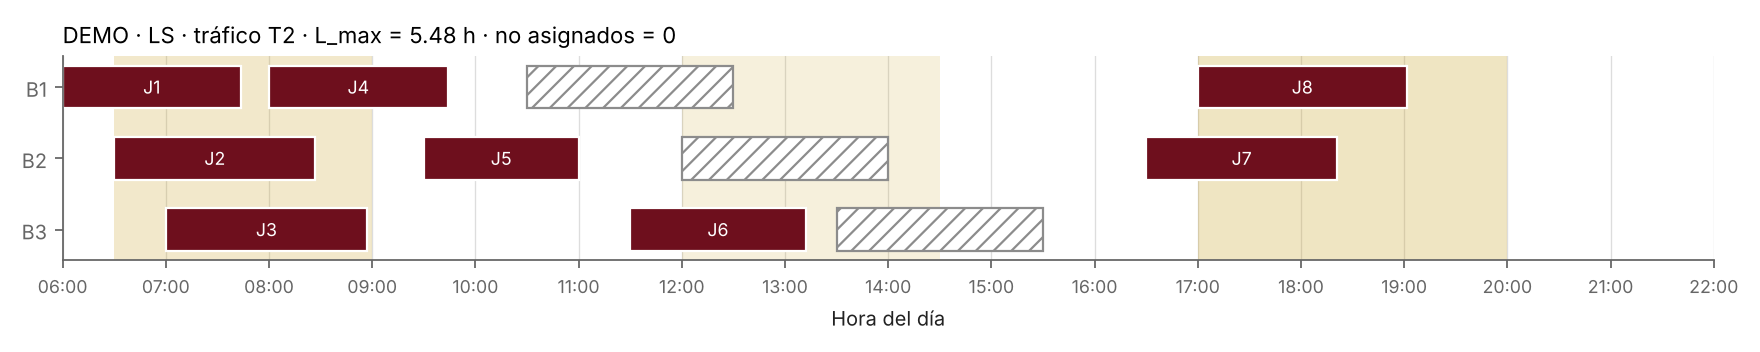
\includegraphics[width=\textwidth]{figuras/fig_gantt_manual_LS_T2.png}
\caption{Programa de List Scheduling (T2). Fondo dorado: franjas de congestión; rayado: almuerzo.}\label{fig:gantt-ls}
\end{figure}
\begin{figure}[H]
\centering
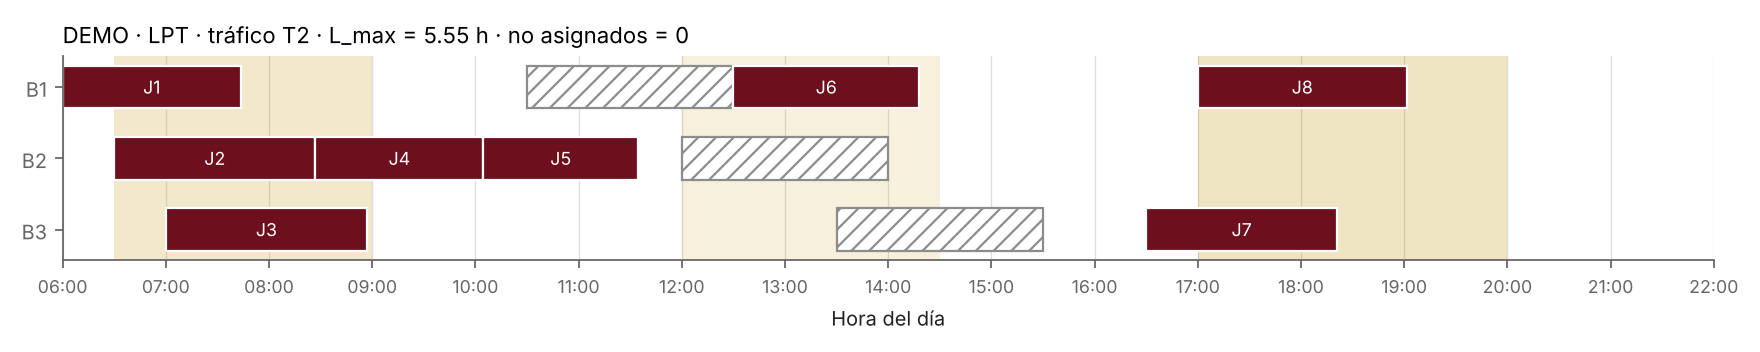
\includegraphics[width=\textwidth]{figuras/fig_gantt_manual_LPT_T2.png}
\caption{Programa de LPT (T2).}\label{fig:gantt-lpt}
\end{figure}

Ambas estrategias atienden las 8 vueltas. Sin tráfico obtienen la misma carga máxima (270\,min, con 3 + 3 + 2 vueltas de 90\,min). Con tráfico, LS obtiene una carga máxima menor (329.0 frente a 333.2\,min). LPT toma primero las vueltas largas de la tarde y reparte las puntas sin seguir el orden temporal; al final, J6 solo cabe en B1 después de su almuerzo. Este resultado y la asignación de cada vuelta coinciden con la salida de \texttt{python -m bus\_sched demo --traffic T2} y con la hoja \emph{Instancia manual} del Excel.

\captura[7cm]{demo_manual_T2.png}{Salida de \texttt{python -m bus\_sched demo --traffic T2} (instancia manual con LS y LPT).}{fig:cap-demo}

\captura[6cm]{excel_instancia_manual.png}{Hoja \emph{Instancia manual} del Excel con las asignaciones de LS y LPT.}{fig:cap-excel-manual}
